% =============================================================================
% fig_ecc_flow.tex  —  TikZ sequence diagram for ECC P-256 counterpart
% Include in main.tex with:  % =============================================================================
% fig_ecc_flow.tex  —  TikZ sequence diagram for ECC P-256 counterpart
% Include in main.tex with:  % =============================================================================
% fig_ecc_flow.tex  —  TikZ sequence diagram for ECC P-256 counterpart
% Include in main.tex with:  % =============================================================================
% fig_ecc_flow.tex  —  TikZ sequence diagram for ECC P-256 counterpart
% Include in main.tex with:  \input{figures/fig_ecc_flow}
% =============================================================================
\begin{figure*}[!t]
\centering
\resizebox{0.92\textwidth}{!}{%
\begin{tikzpicture}[
  >=stealth,
  entity/.style={rectangle, draw, fill=red!10, minimum width=2.2cm,
                 minimum height=0.7cm, font=\small\bfseries},
  msg/.style={->, thick},
  label/.style={font=\footnotesize, midway, above, sloped},
  note/.style={font=\scriptsize, text=gray}
]

% ---- Entities ----
\node[entity] (U)  at (0,0)    {User ($\mathcal{U}$)};
\node[entity] (CS) at (7,0)    {Cloud Server ($\mathcal{CS}$)};

% ---- Lifelines ----
\draw[dashed, gray!60] (U.south)  -- ++(0,-13);
\draw[dashed, gray!60] (CS.south) -- ++(0,-13);

% -------- REGISTRATION PHASE ---------
\node[font=\small\bfseries, fill=green!10, rounded corners, draw=green!60,
      minimum width=4cm] at (3.5,-0.8) {Registration Phase};

\node[font=\scriptsize, align=right, anchor=east] at (-0.2,-1.5)
  {Generate long-term key pair $(d_U, Q_U = d_U \cdot G)$};
% U -> CS
\draw[msg] (0,-2.0) -- (7,-2.0)
  node[label] {$(\ID_U, Q_U)$};
\node[font=\scriptsize, align=left, anchor=west] at (7.2,-2.5)
  {Store $(\ID_U, Q_U)$; generate $(d_S, Q_S)$};
% CS -> U
\draw[msg] (7,-3.0) -- (0,-3.0)
  node[label] {$(Q_S)$};

% -------- LOGIN \& KEY AGREEMENT PHASE ---------
\node[font=\small\bfseries, fill=orange!10, rounded corners, draw=orange!60,
      minimum width=4cm] at (3.5,-3.7) {Login \& Key Agreement Phase};

% U side computations
\node[font=\scriptsize, align=right, anchor=east] at (-0.2,-4.3)
  {Pick ephemeral $e_U \xleftarrow{\$} \mathbb{Z}_n^*$};
\node[font=\scriptsize, align=right, anchor=east] at (-0.2,-4.7)
  {$P_U = e_U \cdot G$ \quad (ephemeral pub key)};
\node[font=\scriptsize, align=right, anchor=east] at (-0.2,-5.1)
  {Pick nonce $N_i \xleftarrow{\$} \{0,1\}^{128}$};
\node[font=\scriptsize, align=right, anchor=east] at (-0.2,-5.5)
  {$V_i = h(\ID_U \| N_i \| P_U \| TS_1)$};

% M1: U -> CS   [936 bits]
\draw[msg] (0,-6.0) -- (7,-6.0)
  node[label] {$M_1 = (P_U,\, N_i,\, TS_1,\, V_i)$\quad\small[936 bits]};

% CS side
\node[font=\scriptsize, align=left, anchor=west] at (7.2,-6.6)
  {Verify $V_i$; check $TS_1$ freshness};
\node[font=\scriptsize, align=left, anchor=west] at (7.2,-7.0)
  {Pick ephemeral $e_S \xleftarrow{\$} \mathbb{Z}_n^*$};
\node[font=\scriptsize, align=left, anchor=west] at (7.2,-7.4)
  {$P_S = e_S \cdot G$};
\node[font=\scriptsize, align=left, anchor=west] at (7.2,-7.8)
  {$Z = e_S \cdot P_U$ \quad (ECDH shared point)};
\node[font=\scriptsize, align=left, anchor=west] at (7.2,-8.2)
  {$\SK = h(Z \| N_i \| N_c \| \ID_U \| \ID_{cs})$};
\node[font=\scriptsize, align=left, anchor=west] at (7.2,-8.6)
  {$V_j = h(\ID_{cs} \| N_c \| P_S \| \SK \| TS_2)$};

% M2: CS -> U   [936 bits]
\draw[msg] (7,-9.1) -- (0,-9.1)
  node[label] {$M_2 = (P_S,\, N_c,\, TS_2,\, V_j)$\quad\small[936 bits]};

% -------- VERIFICATION ---------
\node[font=\small\bfseries, fill=purple!10, rounded corners, draw=purple!60,
      minimum width=4cm] at (3.5,-9.8) {Verification Phase};

\node[font=\scriptsize, align=right, anchor=east] at (-0.2,-10.4)
  {$Z = e_U \cdot P_S$ \quad (same ECDH point)};
\node[font=\scriptsize, align=right, anchor=east] at (-0.2,-10.8)
  {$\SK = h(Z \| N_i \| N_c \| \ID_U \| \ID_{cs})$};
\node[font=\scriptsize, align=right, anchor=east] at (-0.2,-11.2)
  {Verify $V_j$; accept if valid};

% Both hold SK
\node[font=\scriptsize\bfseries, fill=yellow!20, rounded corners, draw=yellow!60]
  at (0,-12.0) {Holds $\SK$};
\node[font=\scriptsize\bfseries, fill=yellow!20, rounded corners, draw=yellow!60]
  at (7,-12.0) {Holds $\SK$};
\draw[<->, double, thick, green!60!black] (0.5,-12.0) -- (6.5,-12.0)
  node[midway, above, font=\scriptsize\bfseries] {Mutual Auth.\ + FS \checkmark};

% Communication note
\node[note, align=center] at (3.5,-13.1)
  {Total: $936 + 936 = 1{,}872$ bits.
   Forward secrecy via ephemeral ECDH~\cite{RFC8446}.};

\end{tikzpicture}%
}
\caption{Message-flow diagram for the ECC P-256 counterpart protocol.
Ephemeral ECDH key pairs $(e_U, P_U)$ and $(e_S, P_S)$ are discarded after
each session, providing forward secrecy. Total communication overhead is
1,872 bits, approximately 2.3$\times$ lower than the Hash+XOR skeleton
(4,224 bits) due to the use of compact nonces.}
\label{fig:ecc_flow}
\end{figure*}

% =============================================================================
\begin{figure*}[!t]
\centering
\resizebox{0.92\textwidth}{!}{%
\begin{tikzpicture}[
  >=stealth,
  entity/.style={rectangle, draw, fill=red!10, minimum width=2.2cm,
                 minimum height=0.7cm, font=\small\bfseries},
  msg/.style={->, thick},
  label/.style={font=\footnotesize, midway, above, sloped},
  note/.style={font=\scriptsize, text=gray}
]

% ---- Entities ----
\node[entity] (U)  at (0,0)    {User ($\mathcal{U}$)};
\node[entity] (CS) at (7,0)    {Cloud Server ($\mathcal{CS}$)};

% ---- Lifelines ----
\draw[dashed, gray!60] (U.south)  -- ++(0,-13);
\draw[dashed, gray!60] (CS.south) -- ++(0,-13);

% -------- REGISTRATION PHASE ---------
\node[font=\small\bfseries, fill=green!10, rounded corners, draw=green!60,
      minimum width=4cm] at (3.5,-0.8) {Registration Phase};

\node[font=\scriptsize, align=right, anchor=east] at (-0.2,-1.5)
  {Generate long-term key pair $(d_U, Q_U = d_U \cdot G)$};
% U -> CS
\draw[msg] (0,-2.0) -- (7,-2.0)
  node[label] {$(\ID_U, Q_U)$};
\node[font=\scriptsize, align=left, anchor=west] at (7.2,-2.5)
  {Store $(\ID_U, Q_U)$; generate $(d_S, Q_S)$};
% CS -> U
\draw[msg] (7,-3.0) -- (0,-3.0)
  node[label] {$(Q_S)$};

% -------- LOGIN \& KEY AGREEMENT PHASE ---------
\node[font=\small\bfseries, fill=orange!10, rounded corners, draw=orange!60,
      minimum width=4cm] at (3.5,-3.7) {Login \& Key Agreement Phase};

% U side computations
\node[font=\scriptsize, align=right, anchor=east] at (-0.2,-4.3)
  {Pick ephemeral $e_U \xleftarrow{\$} \mathbb{Z}_n^*$};
\node[font=\scriptsize, align=right, anchor=east] at (-0.2,-4.7)
  {$P_U = e_U \cdot G$ \quad (ephemeral pub key)};
\node[font=\scriptsize, align=right, anchor=east] at (-0.2,-5.1)
  {Pick nonce $N_i \xleftarrow{\$} \{0,1\}^{128}$};
\node[font=\scriptsize, align=right, anchor=east] at (-0.2,-5.5)
  {$V_i = h(\ID_U \| N_i \| P_U \| TS_1)$};

% M1: U -> CS   [936 bits]
\draw[msg] (0,-6.0) -- (7,-6.0)
  node[label] {$M_1 = (P_U,\, N_i,\, TS_1,\, V_i)$\quad\small[936 bits]};

% CS side
\node[font=\scriptsize, align=left, anchor=west] at (7.2,-6.6)
  {Verify $V_i$; check $TS_1$ freshness};
\node[font=\scriptsize, align=left, anchor=west] at (7.2,-7.0)
  {Pick ephemeral $e_S \xleftarrow{\$} \mathbb{Z}_n^*$};
\node[font=\scriptsize, align=left, anchor=west] at (7.2,-7.4)
  {$P_S = e_S \cdot G$};
\node[font=\scriptsize, align=left, anchor=west] at (7.2,-7.8)
  {$Z = e_S \cdot P_U$ \quad (ECDH shared point)};
\node[font=\scriptsize, align=left, anchor=west] at (7.2,-8.2)
  {$\SK = h(Z \| N_i \| N_c \| \ID_U \| \ID_{cs})$};
\node[font=\scriptsize, align=left, anchor=west] at (7.2,-8.6)
  {$V_j = h(\ID_{cs} \| N_c \| P_S \| \SK \| TS_2)$};

% M2: CS -> U   [936 bits]
\draw[msg] (7,-9.1) -- (0,-9.1)
  node[label] {$M_2 = (P_S,\, N_c,\, TS_2,\, V_j)$\quad\small[936 bits]};

% -------- VERIFICATION ---------
\node[font=\small\bfseries, fill=purple!10, rounded corners, draw=purple!60,
      minimum width=4cm] at (3.5,-9.8) {Verification Phase};

\node[font=\scriptsize, align=right, anchor=east] at (-0.2,-10.4)
  {$Z = e_U \cdot P_S$ \quad (same ECDH point)};
\node[font=\scriptsize, align=right, anchor=east] at (-0.2,-10.8)
  {$\SK = h(Z \| N_i \| N_c \| \ID_U \| \ID_{cs})$};
\node[font=\scriptsize, align=right, anchor=east] at (-0.2,-11.2)
  {Verify $V_j$; accept if valid};

% Both hold SK
\node[font=\scriptsize\bfseries, fill=yellow!20, rounded corners, draw=yellow!60]
  at (0,-12.0) {Holds $\SK$};
\node[font=\scriptsize\bfseries, fill=yellow!20, rounded corners, draw=yellow!60]
  at (7,-12.0) {Holds $\SK$};
\draw[<->, double, thick, green!60!black] (0.5,-12.0) -- (6.5,-12.0)
  node[midway, above, font=\scriptsize\bfseries] {Mutual Auth.\ + FS \checkmark};

% Communication note
\node[note, align=center] at (3.5,-13.1)
  {Total: $936 + 936 = 1{,}872$ bits.
   Forward secrecy via ephemeral ECDH~\cite{RFC8446}.};

\end{tikzpicture}%
}
\caption{Message-flow diagram for the ECC P-256 counterpart protocol.
Ephemeral ECDH key pairs $(e_U, P_U)$ and $(e_S, P_S)$ are discarded after
each session, providing forward secrecy. Total communication overhead is
1,872 bits, approximately 2.3$\times$ lower than the Hash+XOR skeleton
(4,224 bits) due to the use of compact nonces.}
\label{fig:ecc_flow}
\end{figure*}

% =============================================================================
\begin{figure*}[!t]
\centering
\resizebox{0.92\textwidth}{!}{%
\begin{tikzpicture}[
  >=stealth,
  entity/.style={rectangle, draw, fill=red!10, minimum width=2.2cm,
                 minimum height=0.7cm, font=\small\bfseries},
  msg/.style={->, thick},
  label/.style={font=\footnotesize, midway, above, sloped},
  note/.style={font=\scriptsize, text=gray}
]

% ---- Entities ----
\node[entity] (U)  at (0,0)    {User ($\mathcal{U}$)};
\node[entity] (CS) at (7,0)    {Cloud Server ($\mathcal{CS}$)};

% ---- Lifelines ----
\draw[dashed, gray!60] (U.south)  -- ++(0,-13);
\draw[dashed, gray!60] (CS.south) -- ++(0,-13);

% -------- REGISTRATION PHASE ---------
\node[font=\small\bfseries, fill=green!10, rounded corners, draw=green!60,
      minimum width=4cm] at (3.5,-0.8) {Registration Phase};

\node[font=\scriptsize, align=right, anchor=east] at (-0.2,-1.5)
  {Generate long-term key pair $(d_U, Q_U = d_U \cdot G)$};
% U -> CS
\draw[msg] (0,-2.0) -- (7,-2.0)
  node[label] {$(\ID_U, Q_U)$};
\node[font=\scriptsize, align=left, anchor=west] at (7.2,-2.5)
  {Store $(\ID_U, Q_U)$; generate $(d_S, Q_S)$};
% CS -> U
\draw[msg] (7,-3.0) -- (0,-3.0)
  node[label] {$(Q_S)$};

% -------- LOGIN \& KEY AGREEMENT PHASE ---------
\node[font=\small\bfseries, fill=orange!10, rounded corners, draw=orange!60,
      minimum width=4cm] at (3.5,-3.7) {Login \& Key Agreement Phase};

% U side computations
\node[font=\scriptsize, align=right, anchor=east] at (-0.2,-4.3)
  {Pick ephemeral $e_U \xleftarrow{\$} \mathbb{Z}_n^*$};
\node[font=\scriptsize, align=right, anchor=east] at (-0.2,-4.7)
  {$P_U = e_U \cdot G$ \quad (ephemeral pub key)};
\node[font=\scriptsize, align=right, anchor=east] at (-0.2,-5.1)
  {Pick nonce $N_i \xleftarrow{\$} \{0,1\}^{128}$};
\node[font=\scriptsize, align=right, anchor=east] at (-0.2,-5.5)
  {$V_i = h(\ID_U \| N_i \| P_U \| TS_1)$};

% M1: U -> CS   [936 bits]
\draw[msg] (0,-6.0) -- (7,-6.0)
  node[label] {$M_1 = (P_U,\, N_i,\, TS_1,\, V_i)$\quad\small[936 bits]};

% CS side
\node[font=\scriptsize, align=left, anchor=west] at (7.2,-6.6)
  {Verify $V_i$; check $TS_1$ freshness};
\node[font=\scriptsize, align=left, anchor=west] at (7.2,-7.0)
  {Pick ephemeral $e_S \xleftarrow{\$} \mathbb{Z}_n^*$};
\node[font=\scriptsize, align=left, anchor=west] at (7.2,-7.4)
  {$P_S = e_S \cdot G$};
\node[font=\scriptsize, align=left, anchor=west] at (7.2,-7.8)
  {$Z = e_S \cdot P_U$ \quad (ECDH shared point)};
\node[font=\scriptsize, align=left, anchor=west] at (7.2,-8.2)
  {$\SK = h(Z \| N_i \| N_c \| \ID_U \| \ID_{cs})$};
\node[font=\scriptsize, align=left, anchor=west] at (7.2,-8.6)
  {$V_j = h(\ID_{cs} \| N_c \| P_S \| \SK \| TS_2)$};

% M2: CS -> U   [936 bits]
\draw[msg] (7,-9.1) -- (0,-9.1)
  node[label] {$M_2 = (P_S,\, N_c,\, TS_2,\, V_j)$\quad\small[936 bits]};

% -------- VERIFICATION ---------
\node[font=\small\bfseries, fill=purple!10, rounded corners, draw=purple!60,
      minimum width=4cm] at (3.5,-9.8) {Verification Phase};

\node[font=\scriptsize, align=right, anchor=east] at (-0.2,-10.4)
  {$Z = e_U \cdot P_S$ \quad (same ECDH point)};
\node[font=\scriptsize, align=right, anchor=east] at (-0.2,-10.8)
  {$\SK = h(Z \| N_i \| N_c \| \ID_U \| \ID_{cs})$};
\node[font=\scriptsize, align=right, anchor=east] at (-0.2,-11.2)
  {Verify $V_j$; accept if valid};

% Both hold SK
\node[font=\scriptsize\bfseries, fill=yellow!20, rounded corners, draw=yellow!60]
  at (0,-12.0) {Holds $\SK$};
\node[font=\scriptsize\bfseries, fill=yellow!20, rounded corners, draw=yellow!60]
  at (7,-12.0) {Holds $\SK$};
\draw[<->, double, thick, green!60!black] (0.5,-12.0) -- (6.5,-12.0)
  node[midway, above, font=\scriptsize\bfseries] {Mutual Auth.\ + FS \checkmark};

% Communication note
\node[note, align=center] at (3.5,-13.1)
  {Total: $936 + 936 = 1{,}872$ bits.
   Forward secrecy via ephemeral ECDH~\cite{RFC8446}.};

\end{tikzpicture}%
}
\caption{Message-flow diagram for the ECC P-256 counterpart protocol.
Ephemeral ECDH key pairs $(e_U, P_U)$ and $(e_S, P_S)$ are discarded after
each session, providing forward secrecy. Total communication overhead is
1,872 bits, approximately 2.3$\times$ lower than the Hash+XOR skeleton
(4,224 bits) due to the use of compact nonces.}
\label{fig:ecc_flow}
\end{figure*}

% =============================================================================
\begin{figure*}[!t]
\centering
\resizebox{0.92\textwidth}{!}{%
\begin{tikzpicture}[
  >=stealth,
  entity/.style={rectangle, draw, fill=red!10, minimum width=2.2cm,
                 minimum height=0.7cm, font=\small\bfseries},
  msg/.style={->, thick},
  label/.style={font=\footnotesize, midway, above, sloped},
  note/.style={font=\scriptsize, text=gray}
]

% ---- Entities ----
\node[entity] (U)  at (0,0)    {User ($\mathcal{U}$)};
\node[entity] (CS) at (7,0)    {Cloud Server ($\mathcal{CS}$)};

% ---- Lifelines ----
\draw[dashed, gray!60] (U.south)  -- ++(0,-13);
\draw[dashed, gray!60] (CS.south) -- ++(0,-13);

% -------- REGISTRATION PHASE ---------
\node[font=\small\bfseries, fill=green!10, rounded corners, draw=green!60,
      minimum width=4cm] at (3.5,-0.8) {Registration Phase};

\node[font=\scriptsize, align=right, anchor=east] at (-0.2,-1.5)
  {Generate long-term key pair $(d_U, Q_U = d_U \cdot G)$};
% U -> CS
\draw[msg] (0,-2.0) -- (7,-2.0)
  node[label] {$(\ID_U, Q_U)$};
\node[font=\scriptsize, align=left, anchor=west] at (7.2,-2.5)
  {Store $(\ID_U, Q_U)$; generate $(d_S, Q_S)$};
% CS -> U
\draw[msg] (7,-3.0) -- (0,-3.0)
  node[label] {$(Q_S)$};

% -------- LOGIN \& KEY AGREEMENT PHASE ---------
\node[font=\small\bfseries, fill=orange!10, rounded corners, draw=orange!60,
      minimum width=4cm] at (3.5,-3.7) {Login \& Key Agreement Phase};

% U side computations
\node[font=\scriptsize, align=right, anchor=east] at (-0.2,-4.3)
  {Pick ephemeral $e_U \xleftarrow{\$} \mathbb{Z}_n^*$};
\node[font=\scriptsize, align=right, anchor=east] at (-0.2,-4.7)
  {$P_U = e_U \cdot G$ \quad (ephemeral pub key)};
\node[font=\scriptsize, align=right, anchor=east] at (-0.2,-5.1)
  {Pick nonce $N_i \xleftarrow{\$} \{0,1\}^{128}$};
\node[font=\scriptsize, align=right, anchor=east] at (-0.2,-5.5)
  {$V_i = h(\ID_U \| N_i \| P_U \| TS_1)$};

% M1: U -> CS   [936 bits]
\draw[msg] (0,-6.0) -- (7,-6.0)
  node[label] {$M_1 = (P_U,\, N_i,\, TS_1,\, V_i)$\quad\small[936 bits]};

% CS side
\node[font=\scriptsize, align=left, anchor=west] at (7.2,-6.6)
  {Verify $V_i$; check $TS_1$ freshness};
\node[font=\scriptsize, align=left, anchor=west] at (7.2,-7.0)
  {Pick ephemeral $e_S \xleftarrow{\$} \mathbb{Z}_n^*$};
\node[font=\scriptsize, align=left, anchor=west] at (7.2,-7.4)
  {$P_S = e_S \cdot G$};
\node[font=\scriptsize, align=left, anchor=west] at (7.2,-7.8)
  {$Z = e_S \cdot P_U$ \quad (ECDH shared point)};
\node[font=\scriptsize, align=left, anchor=west] at (7.2,-8.2)
  {$\SK = h(Z \| N_i \| N_c \| \ID_U \| \ID_{cs})$};
\node[font=\scriptsize, align=left, anchor=west] at (7.2,-8.6)
  {$V_j = h(\ID_{cs} \| N_c \| P_S \| \SK \| TS_2)$};

% M2: CS -> U   [936 bits]
\draw[msg] (7,-9.1) -- (0,-9.1)
  node[label] {$M_2 = (P_S,\, N_c,\, TS_2,\, V_j)$\quad\small[936 bits]};

% -------- VERIFICATION ---------
\node[font=\small\bfseries, fill=purple!10, rounded corners, draw=purple!60,
      minimum width=4cm] at (3.5,-9.8) {Verification Phase};

\node[font=\scriptsize, align=right, anchor=east] at (-0.2,-10.4)
  {$Z = e_U \cdot P_S$ \quad (same ECDH point)};
\node[font=\scriptsize, align=right, anchor=east] at (-0.2,-10.8)
  {$\SK = h(Z \| N_i \| N_c \| \ID_U \| \ID_{cs})$};
\node[font=\scriptsize, align=right, anchor=east] at (-0.2,-11.2)
  {Verify $V_j$; accept if valid};

% Both hold SK
\node[font=\scriptsize\bfseries, fill=yellow!20, rounded corners, draw=yellow!60]
  at (0,-12.0) {Holds $\SK$};
\node[font=\scriptsize\bfseries, fill=yellow!20, rounded corners, draw=yellow!60]
  at (7,-12.0) {Holds $\SK$};
\draw[<->, double, thick, green!60!black] (0.5,-12.0) -- (6.5,-12.0)
  node[midway, above, font=\scriptsize\bfseries] {Mutual Auth.\ + FS \checkmark};

% Communication note
\node[note, align=center] at (3.5,-13.1)
  {Total: $936 + 936 = 1{,}872$ bits.
   Forward secrecy via ephemeral ECDH~\cite{RFC8446}.};

\end{tikzpicture}%
}
\caption{Message-flow diagram for the ECC P-256 counterpart protocol.
Ephemeral ECDH key pairs $(e_U, P_U)$ and $(e_S, P_S)$ are discarded after
each session, providing forward secrecy. Total communication overhead is
1,872 bits, approximately 2.3$\times$ lower than the Hash+XOR skeleton
(4,224 bits) due to the use of compact nonces.}
\label{fig:ecc_flow}
\end{figure*}
